\documentclass[10pt,a4paper]{article}

\usepackage[utf8]{inputenc}
\usepackage{hyperref}
\usepackage{polski}
\usepackage{graphicx}
\usepackage{listings}
\usepackage{algorithm}
\usepackage{algorithmic}

\usepackage{hyperref}
\usepackage{amssymb}
\usepackage{multicol}
\usepackage{fancyvrb}

\usepackage{color}

\setlength{\topskip}{0mm} \setlength{\topmargin}{0mm}
\setlength{\oddsidemargin}{0mm} \setlength{\evensidemargin}{0mm}
\setlength{\marginparwidth}{0mm} \setlength{\headsep}{0mm}
\setlength{\headheight}{0mm} \setlength{\textheight}{240mm}
\setlength{\textwidth}{170mm}


\floatname{algorithm}{Algorytm}

\lstset{literate=
  {á}{{\'a}}1 {é}{{\'e}}1 {í}{{\'i}}1 {ó}{{\'o}}1 {ú}{{\'u}}1
  {Á}{{\'A}}1 {É}{{\'E}}1 {Í}{{\'I}}1 {Ó}{{\'O}}1 {Ú}{{\'U}}1
  {à}{{\`a}}1 {è}{{\`e}}1 {ì}{{\`i}}1 {ò}{{\`o}}1 {ù}{{\`u}}1
  {À}{{\`A}}1 {È}{{\'E}}1 {Ì}{{\`I}}1 {Ò}{{\`O}}1 {Ù}{{\`U}}1
  {ä}{{\"a}}1 {ë}{{\"e}}1 {ï}{{\"i}}1 {ö}{{\"o}}1 {ü}{{\"u}}1
  {Ä}{{\"A}}1 {Ë}{{\"E}}1 {Ï}{{\"I}}1 {Ö}{{\"O}}1 {Ü}{{\"U}}1
  {â}{{\^a}}1 {ê}{{\^e}}1 {î}{{\^i}}1 {ô}{{\^o}}1 {û}{{\^u}}1
  {Â}{{\^A}}1 {Ê}{{\^E}}1 {Î}{{\^I}}1 {Ô}{{\^O}}1 {Û}{{\^U}}1
  {Ã}{{\~A}}1 {ã}{{\~a}}1 {Õ}{{\~O}}1 {õ}{{\~o}}1
  {œ}{{\oe}}1 {Œ}{{\OE}}1 {æ}{{\ae}}1 {Æ}{{\AE}}1 {ß}{{\ss}}1
  {ű}{{\H{u}}}1 {Ű}{{\H{U}}}1 {ő}{{\H{o}}}1 {Ő}{{\H{O}}}1
  {ç}{{\c c}}1 {Ç}{{\c C}}1 {ø}{{\o}}1 {å}{{\r a}}1 {Å}{{\r A}}1
  {€}{{\euro}}1 {£}{{\pounds}}1 {«}{{\guillemotleft}}1
  {»}{{\guillemotright}}1 {ñ}{{\~n}}1 {Ñ}{{\~N}}1 {¿}{{?`}}1
  {ł}{\l{}}1
}

\definecolor{mygreen}{rgb}{0,0.6,0}
\definecolor{mygray}{rgb}{0.5,0.5,0.5}
\definecolor{mymauve}{rgb}{0.58,0,0.82}

\lstset{
	basicstyle=\footnotesize,
	breakatwhitespace=false,
	breaklines=true,
	captionpos=b,
	commentstyle=\color{mygreen},
	extendedchars=true,
	frame=single,
	keepspaces=true,
	keywordstyle=\color{blue},
	language=C,
	morekeywords={private, True, import, public, class,...},
	numbers=left,
	rulecolor=\color{black},
	showspaces=false,
	showstringspaces=false,
	showtabs=false,
	%   stepnumber=2,
	stringstyle=\color{mymauve},
	tabsize=2
}

\endinput


\begin{document}
\pagestyle{empty}

\begin{center}
\textsc{\Huge{Uniwersytet Zielonogórski}}\\
\LARGE{Wydział Informatyki, Elektrotechniki i~Automatyki}\\
\large{Instytut Sterowania i Systemów Informatycznych}\\
\vspace{0.5cm}
\Large{Programowanie Gier 3D -- Projekt}\\
Prowadzący: Dr inż. Marek Sawerwain \\ \vspace{1cm}
\LARGE{Sprawozdanie z projektu}\\

\vspace{0.5cm}
\Large{Wykonał: Przemysław Dragańczuk, Grupa dziekańska: 33-INF-SSI-SA} \\

\Large{Data oddania projektu: 23.01.2019}
\vspace{1cm}

\begin{flushleft}
	Ocena: ..........................................
\end{flushleft}

\vspace{1cm}
\end{center}



%
% spis treści
%

\begin{multicols}{2}
	\footnotesize
	\tableofcontents
\end{multicols}

\noindent\makebox[\linewidth]{\rule{0.6\paperwidth}{0.4pt}}

\section{Wprowadzenie}
\label{sec:wprowadzenie}

Celem projektu jest stworzenie gry typu ``Platformer'' w przestrzeni 3D
i z widokiem z pierwszej osoby. Sterowanie odbywa się za pomocą
myszki i  klawiatury. Kamera sterowana jest używając myszki, a postacią sterują
klawisze WASD oraz spacja.

\begin{figure}[hb]
	\centering
	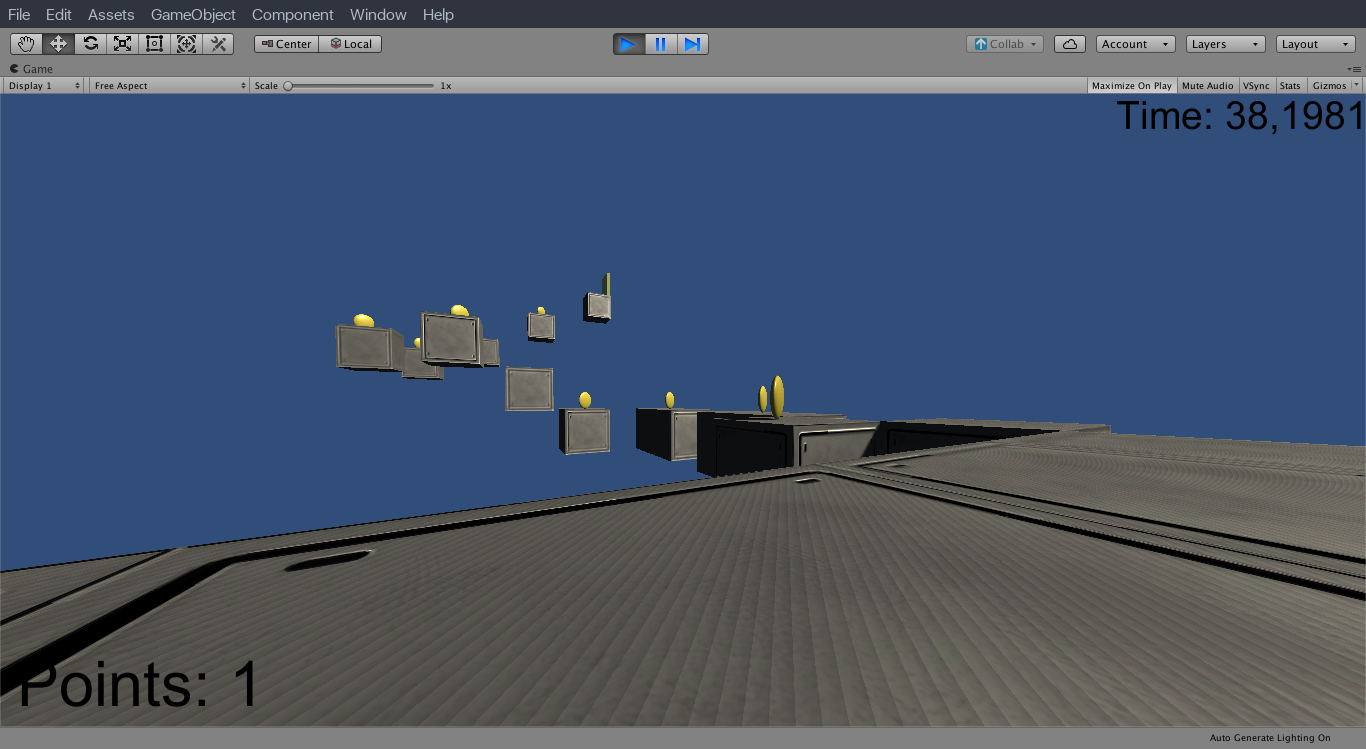
\includegraphics[height=6cm]{screens/lvl.png}
	\label{fig:screen-lvl}
	\caption{Widok z perspektywy postaci}
\end{figure}

\subsection{Planowane funkcjonalności}

\begin{itemize}
	\item Poruszanie postacią
	\item Poruszanie kamerą z perspektywy pierwszej osoby
	\item Skakanie
	\item Przechodzenie między poziomami
	\item Punkty w postaci monet zbieranych przez gracza
	\item Mierzenie czasu, który upłynął od początku poziomu
\end{itemize}


\section{Opis wkładu własnego w realizację projektu}
\subsection{Skrypt zarządzający logiką gry}

Logiką i stanem gry zarządza skrypt \verb`GameLogic`. Zajmuje się on
przechowywaniem takich informacji jak ilość zebranych punktów, obecny
poziom czy czas spędzony w obecnym poziomie. Steruje on również wyświetlaniem
informacji w interfejsie użytkownika.

% Poniżej przedstawiony jest kod tego skryptu:
% \lstinputlisting[language=C]{../Assets/Scripts/GameState.cs}
\subsubsection{Śledzenie punktów}

Śledzenie zebranych punktów odbywa się za pomocą listy obiektów reprezentujących
punkty. Kolizja gracza z danym obiektem oznaczonym jako ``Pickup'' dodaje ten
obiekt do listy, a następnie wyłącza go. W przypadku śmierci gracza, wszystkie
zebrane obiekty są uruchamiane, a lista zostaje opróżniona. W przypadku, gdy
gracz dojdzie do końca poziomu, ilość punktów zostaje dodana do zmiennej
\verb`oldPoints`, a lista zostaje opróżniona. Jako część interfejsu
użytkownika zostaje wyświetlona suma punktów zebranych w poprzednich poziomach
oraz ilości obiektów w liście.

\subsubsection{Zmiana poziomów}

Kolizja gracza z obiektem oznaczonym jako ``Finish'' powoduje przejście do nowego
poziomu. Oznacza to wykonanie kilku czynności. Po pierwsze, następuje sumowanie
punktów opisane wyżej. Następnie usuwany jest obiekt reprezentujący obecny
poziom, a na jego miejsce instancjonowany i aktywowany jest obiekt reprezentujący
następny poziom, który wybierany jest z listy Prefabów. Na końcu resetowany jest
czas spędzony w poziomie.

Prefab reprezentujący poziom musi zawierać:
\begin{itemize}
	\item Znacznik pozycji początkowej, czyli pusty obiekt oznaczony jako ``Start''
	\item Platformy, po których porusza się gracz, oznaczone jako ``Terrain''
	\item Obiekt reprezentujący koniec poziomu, oznaczony jako ``Finish''
\end{itemize}
Dodatkowo powinien zawierać również obiekty reprezentujące punkty, oznaczone
jako ``Pickup''.

Dla wszystkich tych elementów dostępny jest Prefab, zawierający odpowiednie
oznaczenia.

\subsection{Skrypt kontrolujący ruch gracza}

Poruszanie się gracza odbywa się za pomocą zmodyfikowanego skryptu, będącego
portem kodu z gry  (\ref{sec:quake-movement})
 Modyfikacje miały na celu usunięcie funkcjonalności nie używanej
w tym projekcie, dodanie funkcjonalności takich jak prawidłowe ustawianie
pozycji startowej, a także poprawę czytelności kodu.

Na początku gry, a także przy przejściu do następnego poziomu, pozycja gracza
ustawiana jest w zależności od początkowej pozycji ustalonej dla każdego poziomu
jako pusty obiekt. W przypadku, gdy gracz spadnie z mapy, jego pozycja jest
również resetowana.

% \lstinputlisting[language=C]{../Assets/Scripts/PlayerController.cs}

\section{Spis zastosowanych zasobów}
\subsection{Tekstury}
W projekcie została użyta tekstura autorstwa użytkownika ``Spiney'' ze strony
\href{https://opengameart.org}, a konkretnie tekstura i mapa normalnych
``mtl\textunderscore o''
z \href{https://opengameart.org/content/metalstone-textures}{tej paczki}\footnote{https://opengameart.org/content/metalstone-textures}. Użyta
została jako tekstura platform na mapie.

\begin{figure}[ht]
	\centering
	
\includegraphics[height=5cm]{../Assets/Textures/mtl_o_s.png}
	\label{fig:mtlo}
	\caption{Użyta tekstura}
\end{figure}

\subsection{Skrypt kontrolujący ruch gracza}\label{sec:quake-movement}

Skrypt kontrolujący ruch gracza został pobrany z
\href{https://github.com/WiggleWizard/quake3-movement-unity3d}{tego repozytorium}
\footnote{https://github.com/WiggleWizard/quake3-movement-unity3d}.
Skrypt ten jest bezpośrednim portem systemu poruszania w grze Quake 3. Oryginalny
kod z Quake 3 używa licencji GPL-2.0, zatem jego port również jej używa. Co za
tym idzie, zmodyfikowany skrypt używany w tym projekcie także używa tej
licencji.

\section{Podsumowanie}
W trackie trwania projektu udało się zaimplementować prostą, lecz grywalną grę
typu ``Platformer''. Dzięki zaimplementowanemu systemowi zmiany poziomu,
dodawanie nowych map jest proste, a wbudowany pomiar czasu w połączeniu ze
zdobywaniem punktów ma szansę na zainteresowanie społeczności speedrunerskiej.

W projekcie udało się zaimplementować wszystkie planowane funkcjonalności.
\end{document}
